\section{Figures}
    Including the following line in your preamble

    \begin{minted}{latex}
    \DeclareGraphicsExtensions{.png, .jpg, .pdf}
    \end{minted}

    you tell tex to check for graphics in that order. In other words, 
    by not supplying an extension to  \mintinline{latex}{\includegraphics{./figname}}, tex will automatically choose .png before .pdf or .tikz.
    You can later change the priority order if you want. 

    A second or additional, alternative is to order your graphics into different folders.
    ./figs/pdf/, ./figs/pgf/, ./figs/png/,  ./figfs/tikz/, and add to your preamble
    
    \begin{minted}{latex}
    \graphicspath{{./figs/pics/}{./figs/pdf/}}
    \end{minted}

    The code above will tell tex to look for figures in ./figs/pics/ and ./figs/pdf/.
    You can then either supply

    \begin{minted}{latex}
        \includegraphics{some_fig}
    \end{minted}

    which tex will look for in the mentioned folders, in prioritized format. 

    or

    \begin{minted}{latex}
        \includegraphics{absolute/path/to/figure.jpg}
    \end{minted}

            




    \begin{figure}[htbp]
        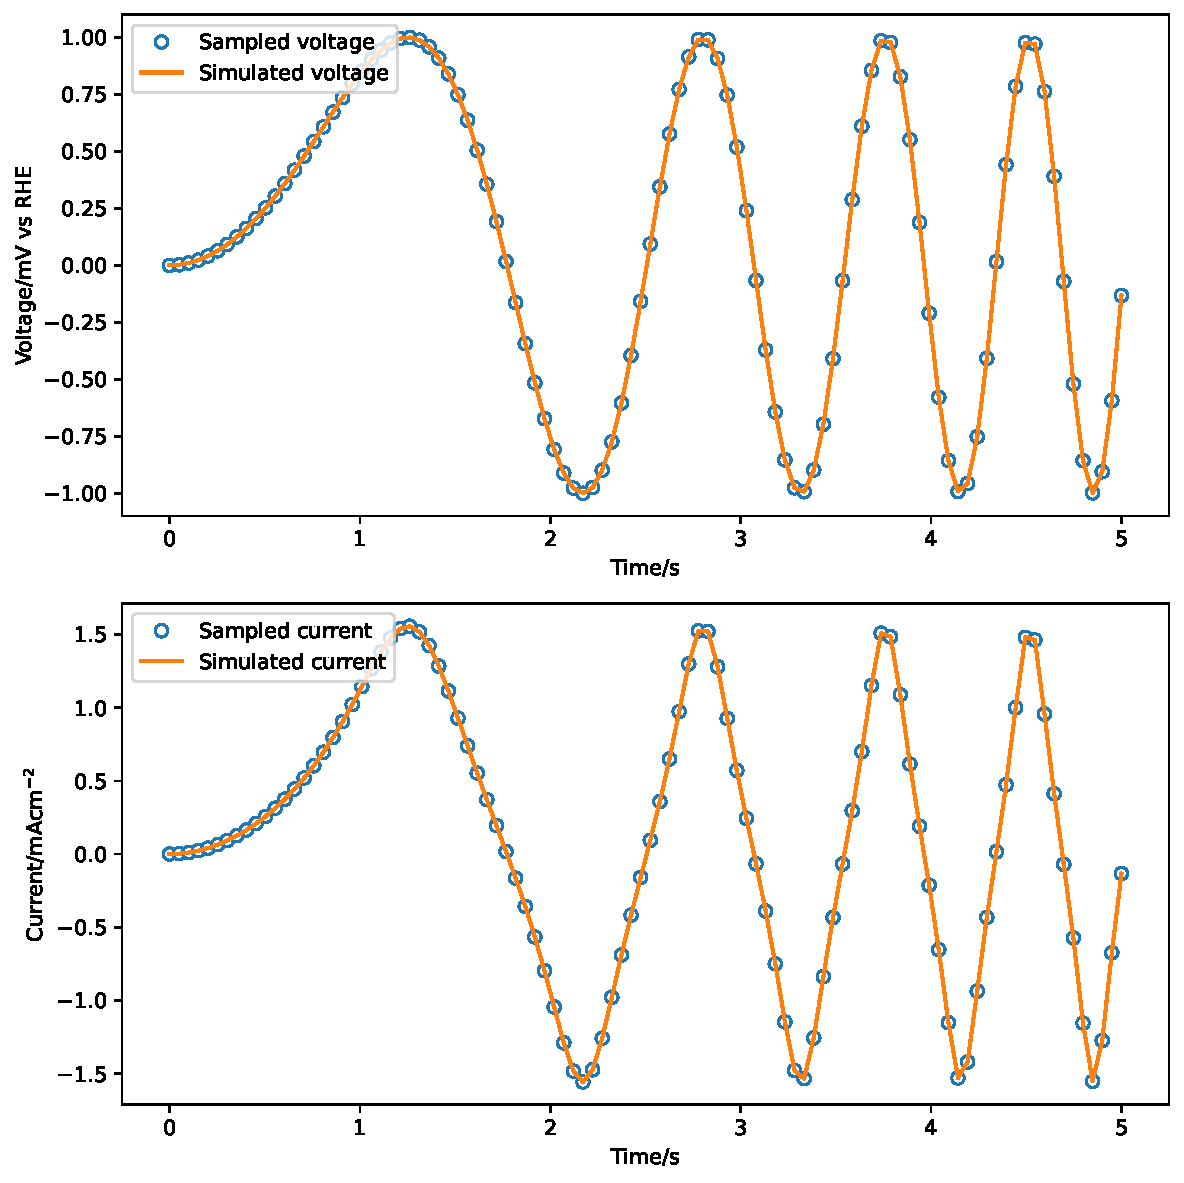
\includegraphics[width=\textwidth]{./figs/example_1.pdf}
        \caption{Figure example included withour file extension}
        \label{figures:fig:example:1}
    \end{figure}

    % You can still specify an extension if you like. This was done in \cref{figures:fig:example:2}. 
    % Notice the difference between \cref{figures:fig:example:2:png,figures:fig:example:2:pdf} and \cref{figures:fig:example:2:pgf,figures:fig:example:tikz}.
    % The former have simply been scaled to width, while the latter has been generatex from pgf and tikz code.

    \begin{figure}
        \begin{subfigure}[t]{0.49\textwidth}
        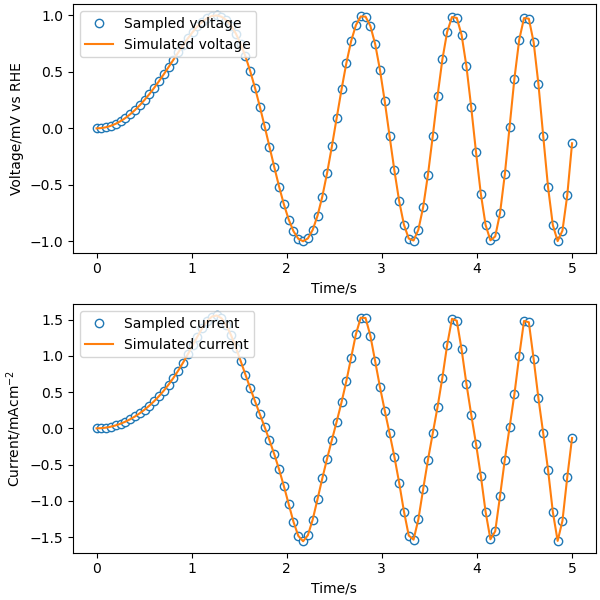
\includegraphics[width=\linewidth]{./figs/example_1.png}
        \caption{.png}
        \label{figures:fig:exmaple:2:png}
        \end{subfigure}
        \hfill
        \begin{subfigure}[t]{0.49\textwidth}
        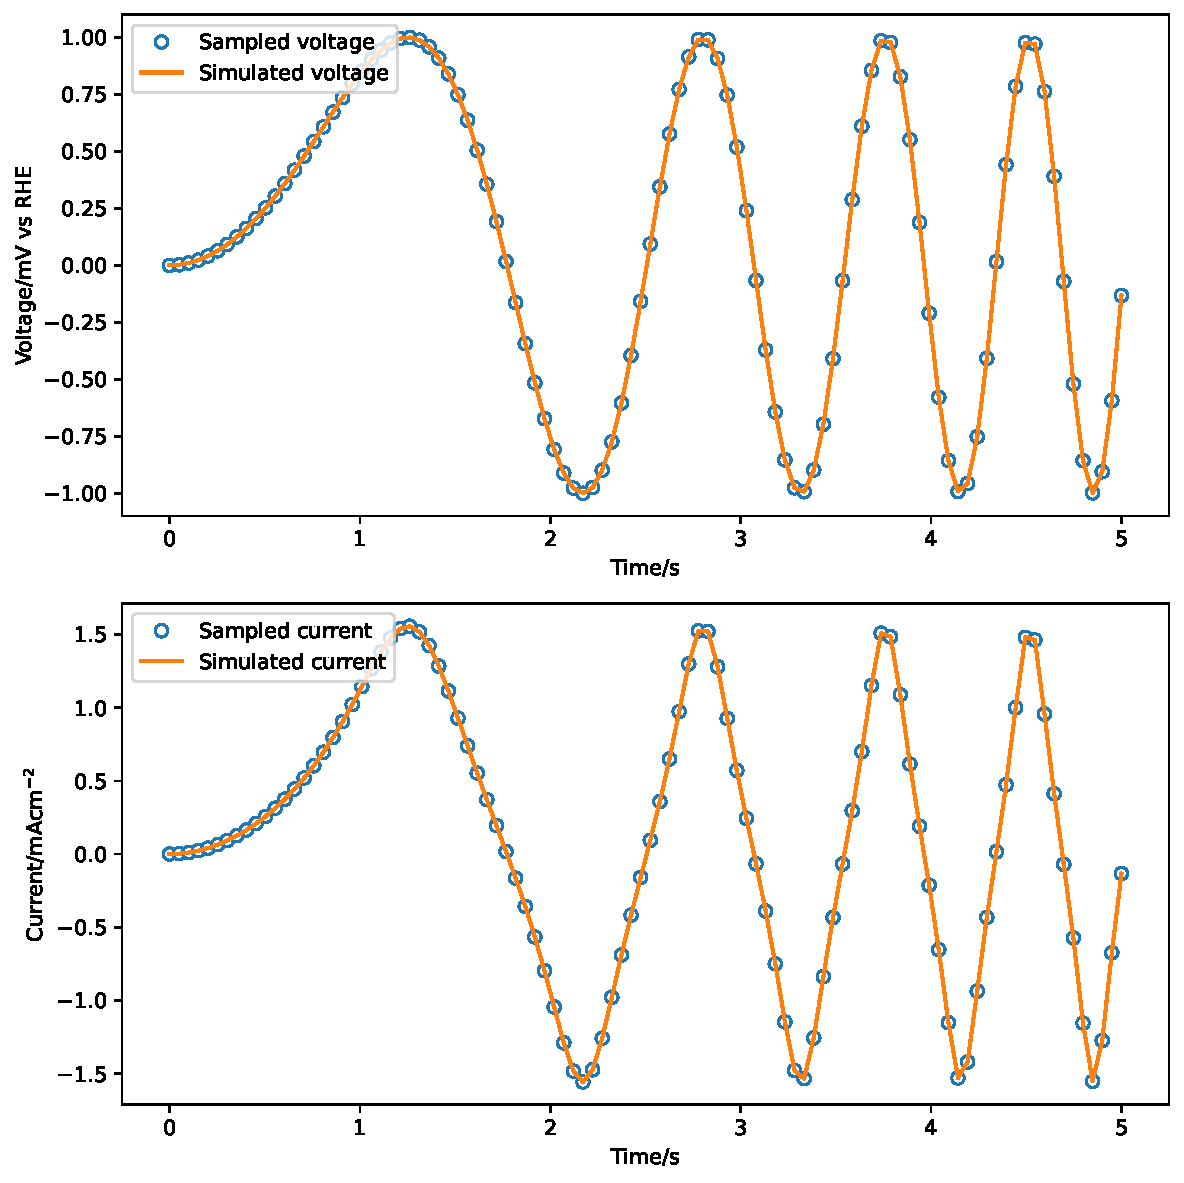
\includegraphics[width=\linewidth]{./figs/example_1.pdf}
        \caption{.pdf}
        \label{figures:fig:exmaple:2:pdf}
        \end{subfigure}
        %
        \begin{subfigure}[t]{0.49\textwidth}
        \includepgf{./figs/example_1.pgf}
        \caption{.pgf}
        \label{figures:fig:exmaple:2:pgf}
         \end{subfigure} 
        \hfill     
        \begin{subfigure}[t]{0.49\textwidth}
        \includetikz{./figs/}{example_1}
        \caption{.tikz}
        \label{figures:fig:exmaple:2:tikz}
        \end{subfigure}     
        \caption{Figures included by specifying file extension.}   
        \label{figures:fig:example:2}
    \end{figure}
